\subsection{由完全割序列生成的理想}

定义 1. 设 A 为环，J 为 A 的理想。若 Ap 的理想 Jp 由一个对 Ap 完全割的序列生成，则称理想 J 在 V(J) 的点 p 处是完全割的。若 J 在 V(J) 的每一点都如此，则称 J 是完全割的。

若 A 的理想 J 是完全割的，则对 A 的每个乘性子集 S，理想 \(S^{-1}J\)（\(S^{-1}A\) 中的）亦然。

每个由完全割序列生成的理想都是完全割的。更精确地：

命题 1.--- 设 A 为环，J 为 \(\Lambda\) 的一个理想，由 A 中元素的有限序列 \(\mathbf{x} = (x_1, \ldots, x_r)\) 生成。下列条件等价：

\begin{enumerate}
\def\labelenumi{(\roman{enumi})}
\item
  序列 x 对 A 是完全割的；
\item
  （相应地 (ii')）对每个素理想（相应地极大理想）\(\mathfrak{p} \in \mathrm{V}(\mathrm{J})\)，\(\mathbf{x}\) 在 \(\mathrm{A}_{\mathfrak{p}}\) 中的像对 \(\mathrm{A}_{\mathfrak{p}}\) 是完全割的；
\item
  （相应地 (iii')）对每个素理想（相应地极大理想）\(\mathfrak{p} \in V(J)\)，理想 J 在 \(\mathfrak{p}\) 处完全割，且 \(x\) 在 \(\kappa(\mathfrak{p})\) -向量空间 \(\kappa(\mathfrak{p}) \otimes_{A} J\) 中的像构成一组基。
\end{enumerate}

当 A 是 Noether 环时，这些条件也等价于：

\begin{enumerate}
\def\labelenumi{(\roman{enumi})}
\setcounter{enumi}{3}
\tightlist
\item
  对每个整数 \(n \geqslant 0\)，A/J-模 \(\mathrm{J}^n/\mathrm{J}^{n+1}\) 是自由的，且单项式 \(x_1^{\alpha_1} \ldots x_r^{\alpha_r}\)（总次数为 \(n\)）的像构成一组基。
\end{enumerate}

设 \(\mathfrak{p}\) 为 A 的一个素理想；记 \(\mathbf{x}_{\mathfrak{p}}\) 为 \(A_{\mathfrak{p}}\) 中序列 \(\mathbf{x}\) 的像。对每个整数 \(i \geqslant 0\)，\(A_{\mathfrak{p}}\) -模 \(H_i(\mathbf{x}_{\mathfrak{p}}, A_{\mathfrak{p}})\) 同构于 \((H_i(\mathbf{x}, A))_{\mathfrak{p}}\) (A, X, 第 151 页, 2))；若 \(\mathfrak{p}\) 不包含 J，则它为零，因为此时有 \(J_{\mathfrak{p}} = A_{\mathfrak{p}}\) (A, X, 第 148 页, 推论 2)。(i)、(ii) 与 (ii') 的等价性由此及 II, § 3, 第 3 节, 定理 1 的推论 2 得出。另一方面，(ii) 与 (iii) 的等价性以及 (ii') 与 (iii') 的等价性由 § 1, 第 3 节, 定理 1 的推论 2 得出。

蕴含关系 (i)⇒(iv) 是 A, X, 第 160 页的定理 1 的推论。最后，条件 (iv) 通过局部化蕴含 \((\mathrm{A}_{\mathfrak{p}}/\mathrm{J}_{\mathfrak{p}})\) -模 \(J_{p}^{n}/J_{p}^{n+1}\) 的类似条件（对每个 \(p \in V(J)\)），而后者由 A, X, 第 160 页的推论 1 蕴含 (ii)。

注.--- 1) 当环 A 是 Noether 环时，在条件 (ii) 与 (ii') 中可把“完全割的”换成“正则的” (A, X, 第 160 页, 推论 1)。

\pandocbounded{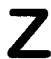
\includegraphics[keepaspectratio]{images/part001_5bbbde23.jpg}}

注意在条件 (i) 中并非如此：一个对 A 完全割的序列未必是 A-正则的 (习题 1)。

\begin{enumerate}
\def\labelenumi{\arabic{enumi})}
\setcounter{enumi}{1}
\tightlist
\item
  设 A 为环，J 为 A 的一个有限生成理想，p 为 A 的一个包含 J 的素理想。由 § 1, 第 3 节的定理 1 的推论 2，有

\[
\operatorname{prof} _ {A _ {\mathfrak {p}}} (J _ {\mathfrak {p}}; A _ {\mathfrak {p}}) \leqslant [ \kappa (\mathfrak {p}) \otimes_ {A} J: \kappa (\mathfrak {p}) ],
\]

且等号成立当且仅当 J 在 p 处完全割。
\end{enumerate}

设 J 异于 A 且由一个完全割序列 \((x_{1},\ldots,x_{r})\) 生成。则有 (§ 1, 第 3 节的命题 4 及上面的命题 1)

\[
\operatorname{prof} _ {A} (J; A) = \inf _ {\mathfrak {p} \in V (J)} \operatorname{prof} _ {A _ {\mathfrak {p}}} (J _ {\mathfrak {p}}; A _ {\mathfrak {p}}) = r.
\]

若进而 A 是 Noether 环，则有 \(\operatorname{codim}(\mathrm{V}(\mathrm{J}),\operatorname{Spec}(\mathrm{A}))\leqslant r\) (VIII, § 3, 第 3 节, 命题 4) 与 \(\operatorname{prof}_{\mathrm{A}}(\mathrm{J};\mathrm{A})\leqslant \operatorname{codim}(\mathrm{V}(\mathrm{J}),\operatorname{Spec}(\Lambda))\) (§ 1, 第 7 节, 命题 12)，从而最终有

\[
\operatorname{prof} _ {\mathrm{A}} (\mathrm{J}; \mathrm{A}) = r = \operatorname{codim} (\mathrm{V} (\mathrm{J}), \operatorname{Spec} (\mathrm{A})) = \operatorname{ht} (\mathrm{J}).
\]

